
\lecture{Probability Rules}{probability-rules}
\section{Probability Rules}

\title{Probability Rules}
\subtitle{Putting it All Together}

%\author{Kelly Black}
%\institute{Clarkson University}
\date{17 January 2014}

\begin{frame}
  \titlepage
\end{frame}

\begin{frame}
  \frametitle{Outline}
  \tableofcontents[hideothersubsections,sectionstyle=show/hide]
\end{frame}


\subsection{Clicker Quiz}


\iftoggle{clicker}{%
  \begin{frame}
    \frametitle{Clicker Quiz}

    I have a bag with ten blue marbles and four red marbles. I remove
    one marble and put it to the side. The marble was a blue
    marble. What is the probability that I pull out a blue marble the
    next time I draw a marble?

    \vspace{2em}

    \begin{tabular}{l@{\hspace{3em}}l@{\hspace{3em}}l@{\hspace{3em}}l}
      A: $\frac{10}{14}$ & B: $\frac{9}{13}$ & C: $\frac{4}{14}$ & D: $\frac{4}{13}$
    \end{tabular}

    \vfill

  \end{frame}
}

\begin{frame}
  \frametitle{Verbiage Issues}

  I have a bag with ten blue marbles and four red marbles. I remove
  one marble \textbf{\color{red}{without replacement}}. The marble was
  a blue marble. What is the probability that I pull out a blue marble
  the next time I draw a marble?

    \vfill

\end{frame}

\begin{frame}{I Know Things}

  Problem: Sometimes I know something about what
  occured. \textit{\textbf{Given}} that information how do I incorporate it
  into the probability that some event occured?

  \vfill
  \includegraphics[width=5cm]{img/vennDiagram}
  \vfill
  
\end{frame}

\begin{frame}
  \frametitle{Example From Last Time}

  1000 voters are polled in the 2008 election. We get the following
  information: \\
  \only<1>
  {
    \begin{tabular}{l|l|l|l}
      Education & Obama & McCain & Others  \\ \hline
      No H.S. Diploma & 19 & 20 & 1   \\
      H.S. Diploma only & 114 & 103 & 3 
    \end{tabular}
  }
  \only<2->
  {
    \begin{tabular}{l|l|l|l|l}
      Education & Obama & McCain & Others & \color{red}{Total} \\ \hline
      No H.S. Diploma & 19 & 20 & 1 & \color{red}{40} \\
      H.S. Diploma only & 114 & 103 & 3 & \color{red}{220} \\ \hline
      \color{red}{Total} & \color{red}{133} & \color{red}{123} & \color{red}{4} & \color{blue}{260}
    \end{tabular}
  }



\end{frame}



\begin{frame}{Conditional Probability}

  I know that B occured. Given that information, what is the
  probability that A occured?

  \begin{definition}{Conditional Probability}

    The probability that A occurs given that I know that B occured is
    denoted by
    \begin{eqnarray*}
      p(A|B).
    \end{eqnarray*}
    
  \end{definition}
  
\end{frame}




\begin{frame}{Conditional Probability}

  \includegraphics[width=5cm]{img/vennDiagram}

  I know that B occured. Given that information, what is the
  probability that A occured?

  
\end{frame}

\begin{frame}
  \frametitle{Conditional Probability}

  \begin{definition}
    The probability that A occurs given that I know that B occured is
    defined to be 
    \begin{eqnarray*}
      p(A|B) & = & \frac{p(A \mathrm{~and~} B)}{p(B)}, \\
      \mathrm{or~} 
      p(B) p(A|B)  &  =  & p(A \mathrm{~and~} B).
    \end{eqnarray*}
  \end{definition}

\end{frame}


\begin{frame}{Example 2}

  I have a bag with eight marbles. Five marbles are red and three are
  blue. I pick two, one after the other without replacing them. What
  is the probability that I pull out a red and then a blue marble?

  \vfill

  \uncover<2->%
  {

    What is the probability that I get exactly one red marble?
    \vfill

  }
  
\end{frame}


\subsection{Probability Rules}

\begin{frame}{Probability Rules}

  \begin{definition}
    The multiplication rule:
    \begin{eqnarray*}
      p(A)\cdot p(B|A) & = & p(A \mathrm{~and~} B), \\
      p(B)\cdot p(A|B) & = & p(A \mathrm{~and~} B).
    \end{eqnarray*}

    The addition rule:
    \begin{eqnarray*}
      p(A \mathrm{~or~} B) & = & p(A) + p(B) - p(A \mathrm{~and~} B).
    \end{eqnarray*}

    The compliment rule:
    \begin{eqnarray*}
      p(A^c) & = & 1 - p(A).
    \end{eqnarray*}

  \end{definition}

  \vfill
  
\end{frame}


\subsection{Examples}

\begin{frame}
  \frametitle{Example 1}

  \vfill

  A ball is hidden under one of three cups. You pay \$5.00 to find the
  ball. You get \$10.00 if you find it on your first guess. You get
  \$2.00 if you get it on your second guess. Otherwise you get
  nothing.

  \vfill

  What is the probability of getting some money back?

  \vfill

\end{frame}


\begin{frame}
  \frametitle{Clicker Quiz}
  
  \vfill

  A store sells skates. Thirty percent of the skates are used. Five
  percent of the new skates are defective. Twenty percent of the used
  skates are defective. You pick one set of skates out at random. What
  is the probability that the set is defective?

  \vfill

  \begin{tabular}{l@{\hspace{3em}}l@{\hspace{3em}}l@{\hspace{3em}}l}
    A: 0.050  & B: .095  & C: .110 & D: .250
  \end{tabular}

  \vfill

\end{frame}


\begin{frame}{Example}

  \vfill

  A test can detect the presence of an abnormal gene that causes cystic
  fibrosis (CF). It is estimated that about 5\% of all people have the
  abnormal gene. The test is correct 90\% of the time for people who
  have the abnormal gene. About 2\% of the time it is positive for
  people who do not have the abnormal gene.

  \vfill

  If someone tests positive for the abnormal gene what is the
  probability that they have the abnormal gene?

  \vfill
  
\end{frame}

\begin{frame}
  \frametitle{Example}

  I have a bag with ten blue marbles and four red marbles. I remove
  two marbles without replacement. What is the probability that I pull
  out at least one blue marble?


  \vfill

\end{frame}



% LocalWords:  Clarkson pausesection hideallsubsections hideothersubsections
% LocalWords:  sectionstyle Obama
